\documentclass[final]{beamer}
\usepackage[size=a0,scale=1]{beamerposter}
\usetheme{ConfPoster} % You can change to other poster themes if you like
\usepackage{graphicx}
\usepackage{subcaption}
\usepackage{amsmath, amssymb}
\usepackage{pifont}  % For handwritten-style cross
\usepackage{tikz}
\usepackage{qrcode}
\usepackage{blkarray} % optional for QR codes
\usepackage{xcolor}
\usepackage{listings}
\usepackage{tabularx}
\usepackage{minted}

\usepackage{setspace}   % control line spacing
\usepackage{parskip}    % automatic paragraph spacing

\let\oldblock\block
\let\endoldblock\endblock

\renewenvironment{block}[1]{%
    \vspace{2em} % space above
    \oldblock{#1}%
    }{%
    \endoldblock   % ends the original block
    \vspace{2em} % space below
}


\newcommand{\cmark}{{\color{green!60!black} \ding{52}}}
\newcommand{\xmark}{\color{red} \ding{56}} % Handwritten-style cross

\title{Qompiler: A Traceable Quantum Circuit Synthesis from Arbitrary Hamiltonians}
\author{Shoupu Wan, PhD \ \texttt{wanshoupu@gmail.com} \ GitHub: \texttt{wanshoupu/quantum-simulations}}
\institute{OpenForJob}

\begin{document}

    \begin{frame}[t]
        \begin{columns}[t]

            % Column 1
            \begin{column}{0.33\textwidth}

                \begin{block}{Introduction}
                    Quantum simulation provides exponential advantages for applications in chemistry, pharmaceuticals, and biological processes.
                    However, quantum software development remains challenging, requiring deep expertise in physics, mathematics, and software engineering.
                    Existing transpilers are often platform-specific and lack flexible control over circuit granularity.

                    To address these challenges, we developed \texttt{Qompiler}—a cross-platform quantum circuit synthesizer that emphasizes traceability,
                    verifiability, and configurable gate selection.
                    It decomposes Hamiltonians using a multi-stage framework and represents the circuits
                    in a platform-independent B-Tree structure that supports gate-level lineage.

                    \texttt{Qompiler} enables hardware-aware circuit generation, supporting major frameworks such as Qiskit, Cirq, and OpenQASM,
                    while allowing users to tailor the gate sets to match the native capabilities of different quantum devices.
                \end{block}


                \begin{block}{Methodology}
                    The \texttt{Qompiler} decomposes user-defined Hamiltonians into executable quantum circuits
                    through a multi-stage decomposition process~\cite{nielsen2010quantum}.
                    Starting from the $n$-dimensional unitary operator,
                    the input operator undergoes a number of decomposition processes
                    until the quantum gates reach the intended granularity.
                    The compiler provides fine-grained control over decomposition granularity and optimization levels
                    to match the native constraints of specific quantum hardware.
                    We have listed the terminology for granularity classification of unitary operators and quantum gates below.


                    \vspace{2em}
                    \begin{tabularx}{.9\textwidth}{lXl}
                        \hline
                        \textbf{Term} & \textbf{Description}                                                           & \textbf{Enum}          \\
                        \hline
                        Unitary       & Any $n$-qubit unitary operator                                                 & \texttt{UNITARY}       \\
                        2level        & Unitary operator with no more than two non-identity rows/columns               & \texttt{TWO\_LEVEL}    \\
                        Multi-Target  & Gates with $2+$ target qubit and any number of control qubits                  & \texttt{MULTI\_TARGET} \\
                        Singlet       & Gates with a single target and any number of control qubits                    & \texttt{SINGLET}       \\
                        Ctrl-pruned   & Controlled gates with a single target and at most one control qubit            & \texttt{CTRL\_PRUNED}  \\
                        Principal     & Single-qubit gates of the form $R_n(\theta)$with $n=x,y,z$                     & \texttt{PRINCIPAL}     \\
                        Universal     & Single-qubit gates in the set $\{X, Y, Z, H, S, T, \mathit{SD}, \mathit{TD}\}$        & \texttt{UNIV\_GATE}    \\
                        Clifford+T    & Gates in the set $\{\mathit{CNOT}, H, S, T\}$                                  & \texttt{CLIFFORD\_T}   \\
                        \hline
                    \end{tabularx}
                    \vspace{2em}


                    When a gate meets the requirements of multiple categories, the finest one is chosen.
                    For example, if a single-target gate has one control qubit a core matrix \texttt{X},
                    we classify it as \texttt{Clifford+T}.
                    The decomposition processes used by \texttt{Qompiler} are listed in the table below.


                    \vspace{2em}
                    \begin{tabularx}{.9\textwidth}{lX}
                        \hline
                        \textbf{Decomposition}        & \textbf{Description}                                                                                                                                        \\
                        \hline
                        \texttt{mat2l\_decompose}     & Decomposes an arbitrary $n \times n$ unitary matrix into \texttt{2level} unitary matrices.                                                                  \\
                        \texttt{cnot\_decompose}      & Decomposes a \texttt{2level} unitary matrix into single-target operators in universal gates.                                                                \\
                        \texttt{ctrl\_decompose}      & Given a controlled gate, breaks its control sequence down to shorter controls, usually with the help of ancilla qubits.                                     \\
                        \texttt{euler\_decompose}     & Decomposes a single-qubit gate into Euler rotation operators and optionally a phase shift.                                                                  \\
                        \texttt{cliffordt\_decompose} & Given a universal gate, decomposes it into \texttt{Clifford+T} gates.                                                                                       \\
                        \texttt{sk\_decompose}        & Based on the Solovay-Kitaev Theorem, approximates a single-qubit gate into \texttt{universal} gates or a subset of it, e.g., the \texttt{Clifford+T} gates. \\
                        \hline
                    \end{tabularx}
                    \vspace{2em}


                    The platform-independent quantum intermediate language (QIL) can be rendered into target-specific circuits
                    for Qiskit, Cirq, and OpenQASM~\cite{openqasm2,openqasm3}. \texttt{Qompiler} allows users to configure
                    the final gate set to align with hardware characteristics—for example, prioritizing Pauli gates
                    ($X$, $Y$, $Z$) for superconducting devices or rotation gates ($R_x(\phi)$, $R_y(\phi)$, $R_z(\phi)$)
                    for trapped-ion platforms such as IonQ. This hardware-aware configurability enables efficient, optimized
                    circuit generation while preserving cross-platform compatibility.


                    To compare \texttt{Qompiler} with existing quantum compilers/transpilers/synthesizers, we select a couple of key features,
                    that is, cross-platform compatibility, gate traceability, and gate customizability.
                    Feature comparison between \texttt{Qompiler} and existing quantum compilation tools in the table below~\cite{tket,quilc,qfast,staq}.
                    A gray check mark is associated with Qiskit for its partial control over the gate types in the end result.


                    \vspace{2em}
                    \begin{tabularx}{.8\textwidth}{X|c|c|c|c|c|c|c}
                        \hline
                        \textbf{Feature}          & \textbf{Qiskit} & \textbf{Tket} & \textbf{Cirq} & \textbf{Quilc} & \textbf{QFast} & \textbf{Staq} & \textbf{Qompiler} \\
                        \hline
                        Cross-platform compatibility         & \cmark          & \cmark        & \cmark        & \xmark         & \xmark         & \cmark        & \cmark \\
                        Gate traceability & \xmark          & \xmark        & \xmark        & \xmark         & \xmark         & \xmark        & \cmark \\
                        Gate customizability    & \textcolor{gray}{\ding{52}} & \xmark & \xmark & \xmark & \cmark & \xmark & \cmark \\
                        \hline
                    \end{tabularx}
                    \vspace{2em}

                \end{block}
            \end{column}

            % Column 2
            \begin{column}{0.33\textwidth}
                \begin{block}{Architecture}

                    Here we provide an overview of the high-level design of `Qompiler'.
                    The system is organized into the following functional parts:
                    ``Compiler configuration'', ``Matrix decomposition'', ``Optimization'', ``Circuit rendering''.


                    \vspace{2em}
                    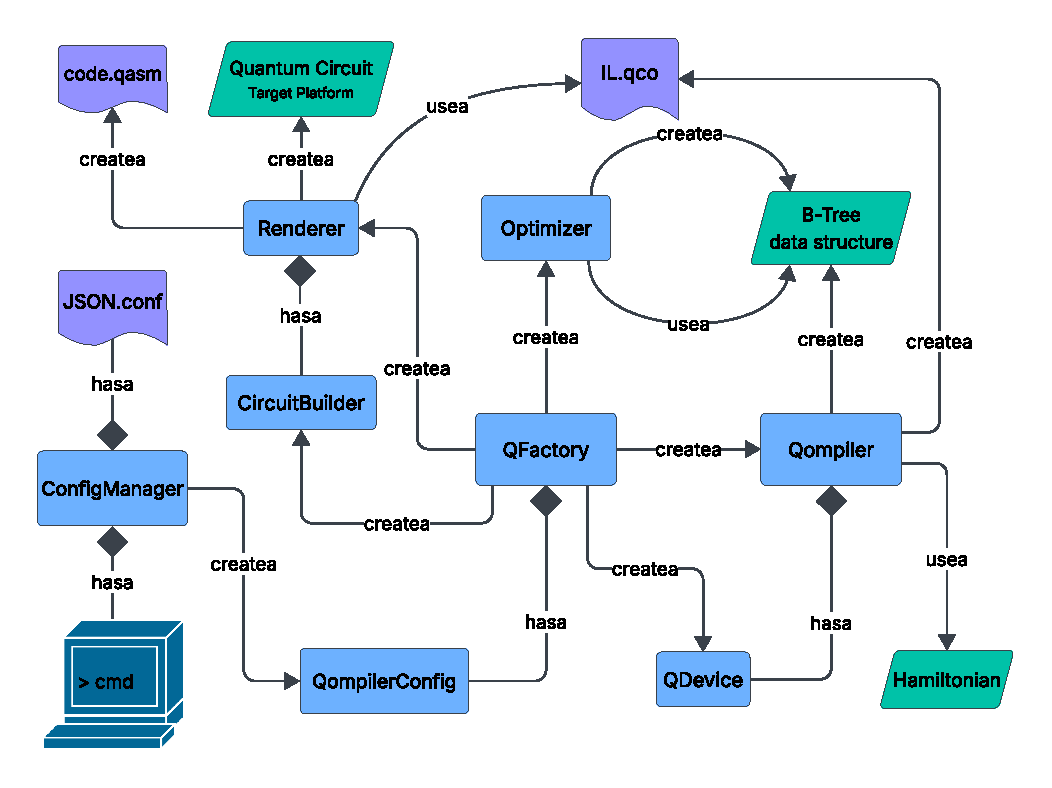
\includegraphics[width=.8\linewidth]{architecture}
                    \vspace{2em}



                    The decomposition workflow and the resulting QIL, a B-Tree data structure, is written to a \textit{.qco} file.

                    \begin{figure}[tbhp]
                        \centering
                        \begin{subfigure}{0.45\textwidth}
                            \centering
                            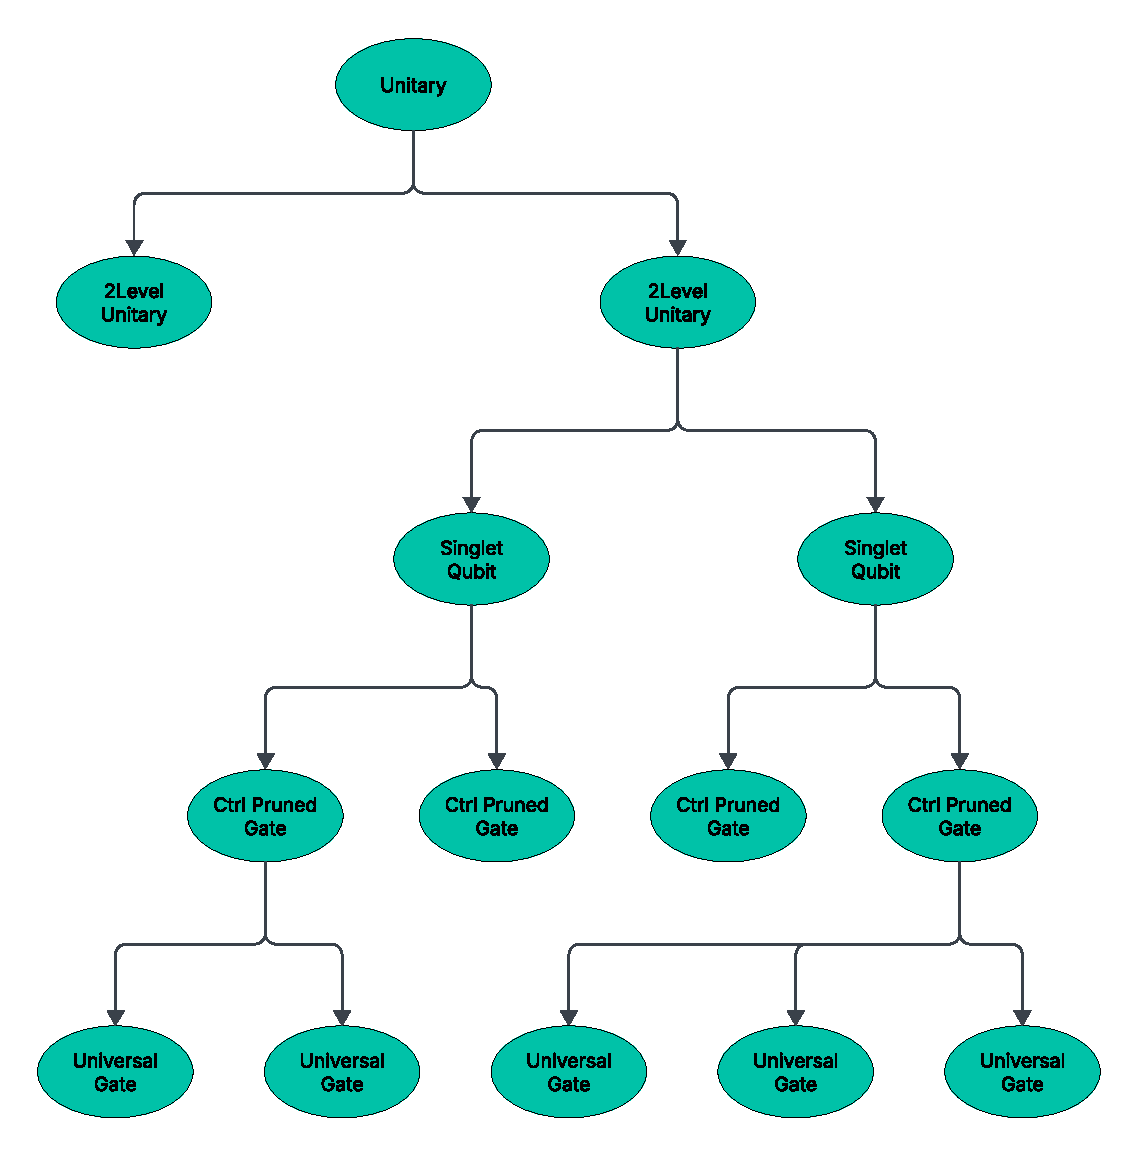
\includegraphics[width=.6\textwidth,scale=0.7]{btree}
                            \caption{Compiled code as a B-Tree data structure.}
                            \label{fig:btree}
                        \end{subfigure}
                        \hfill
                        \begin{subfigure}{0.45\textwidth}
                            \centering
                            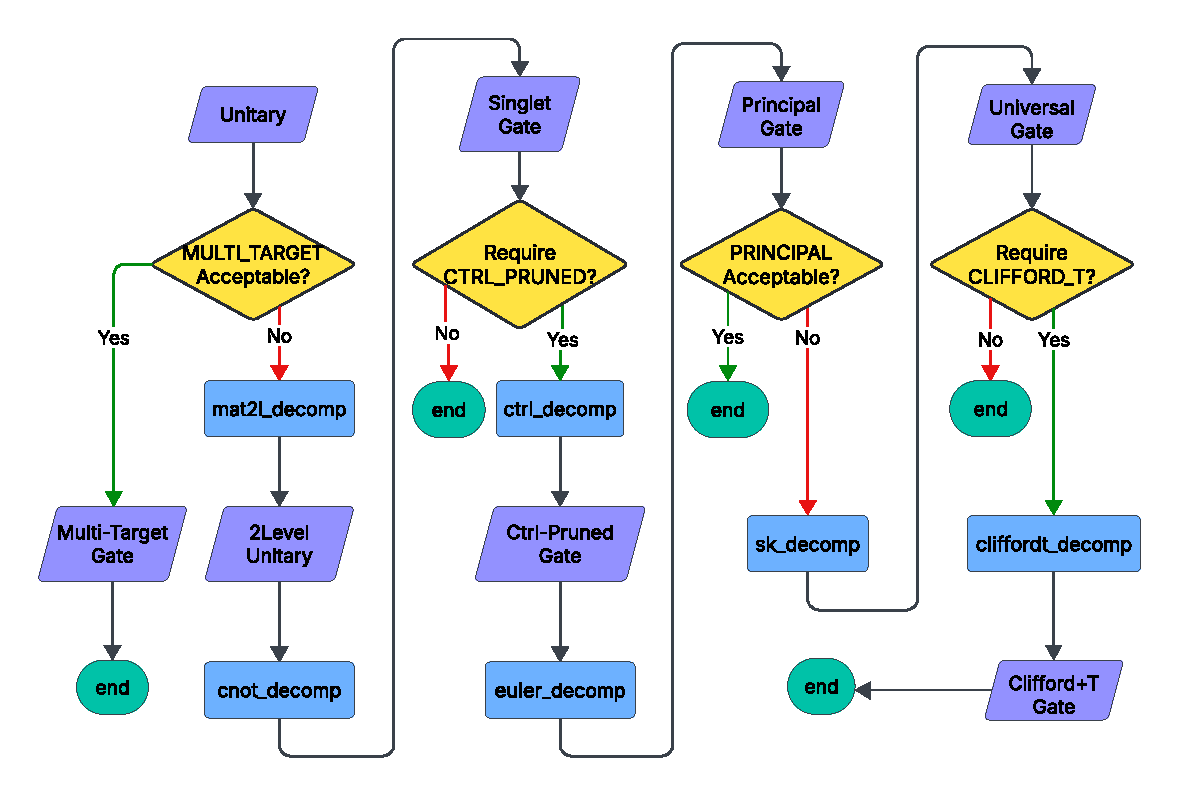
\includegraphics[width=\linewidth]{workflow}
                            \caption{The compilation workflow.}
                            \label{fig:workflow}
                        \end{subfigure}
                        \label{fig:Qompiler}
                    \end{figure}

                \end{block}

                \begin{block}{Results}


                    \begin{figure}[tbhp]
                        \centering
                        \begin{subfigure}{0.45\textwidth}
                            \centering
                            \includegraphics[width=\linewidth,clip,trim=0 13100 0 30]{random-unitary.pdf}
                            \caption{Circuit diagram (partial) in Qiskit\textregistered.}
                            \label{fig:qiskit-circuit}
                        \end{subfigure}
                        \hfill
                        \begin{subfigure}{0.45\textwidth}
                            \centering
                            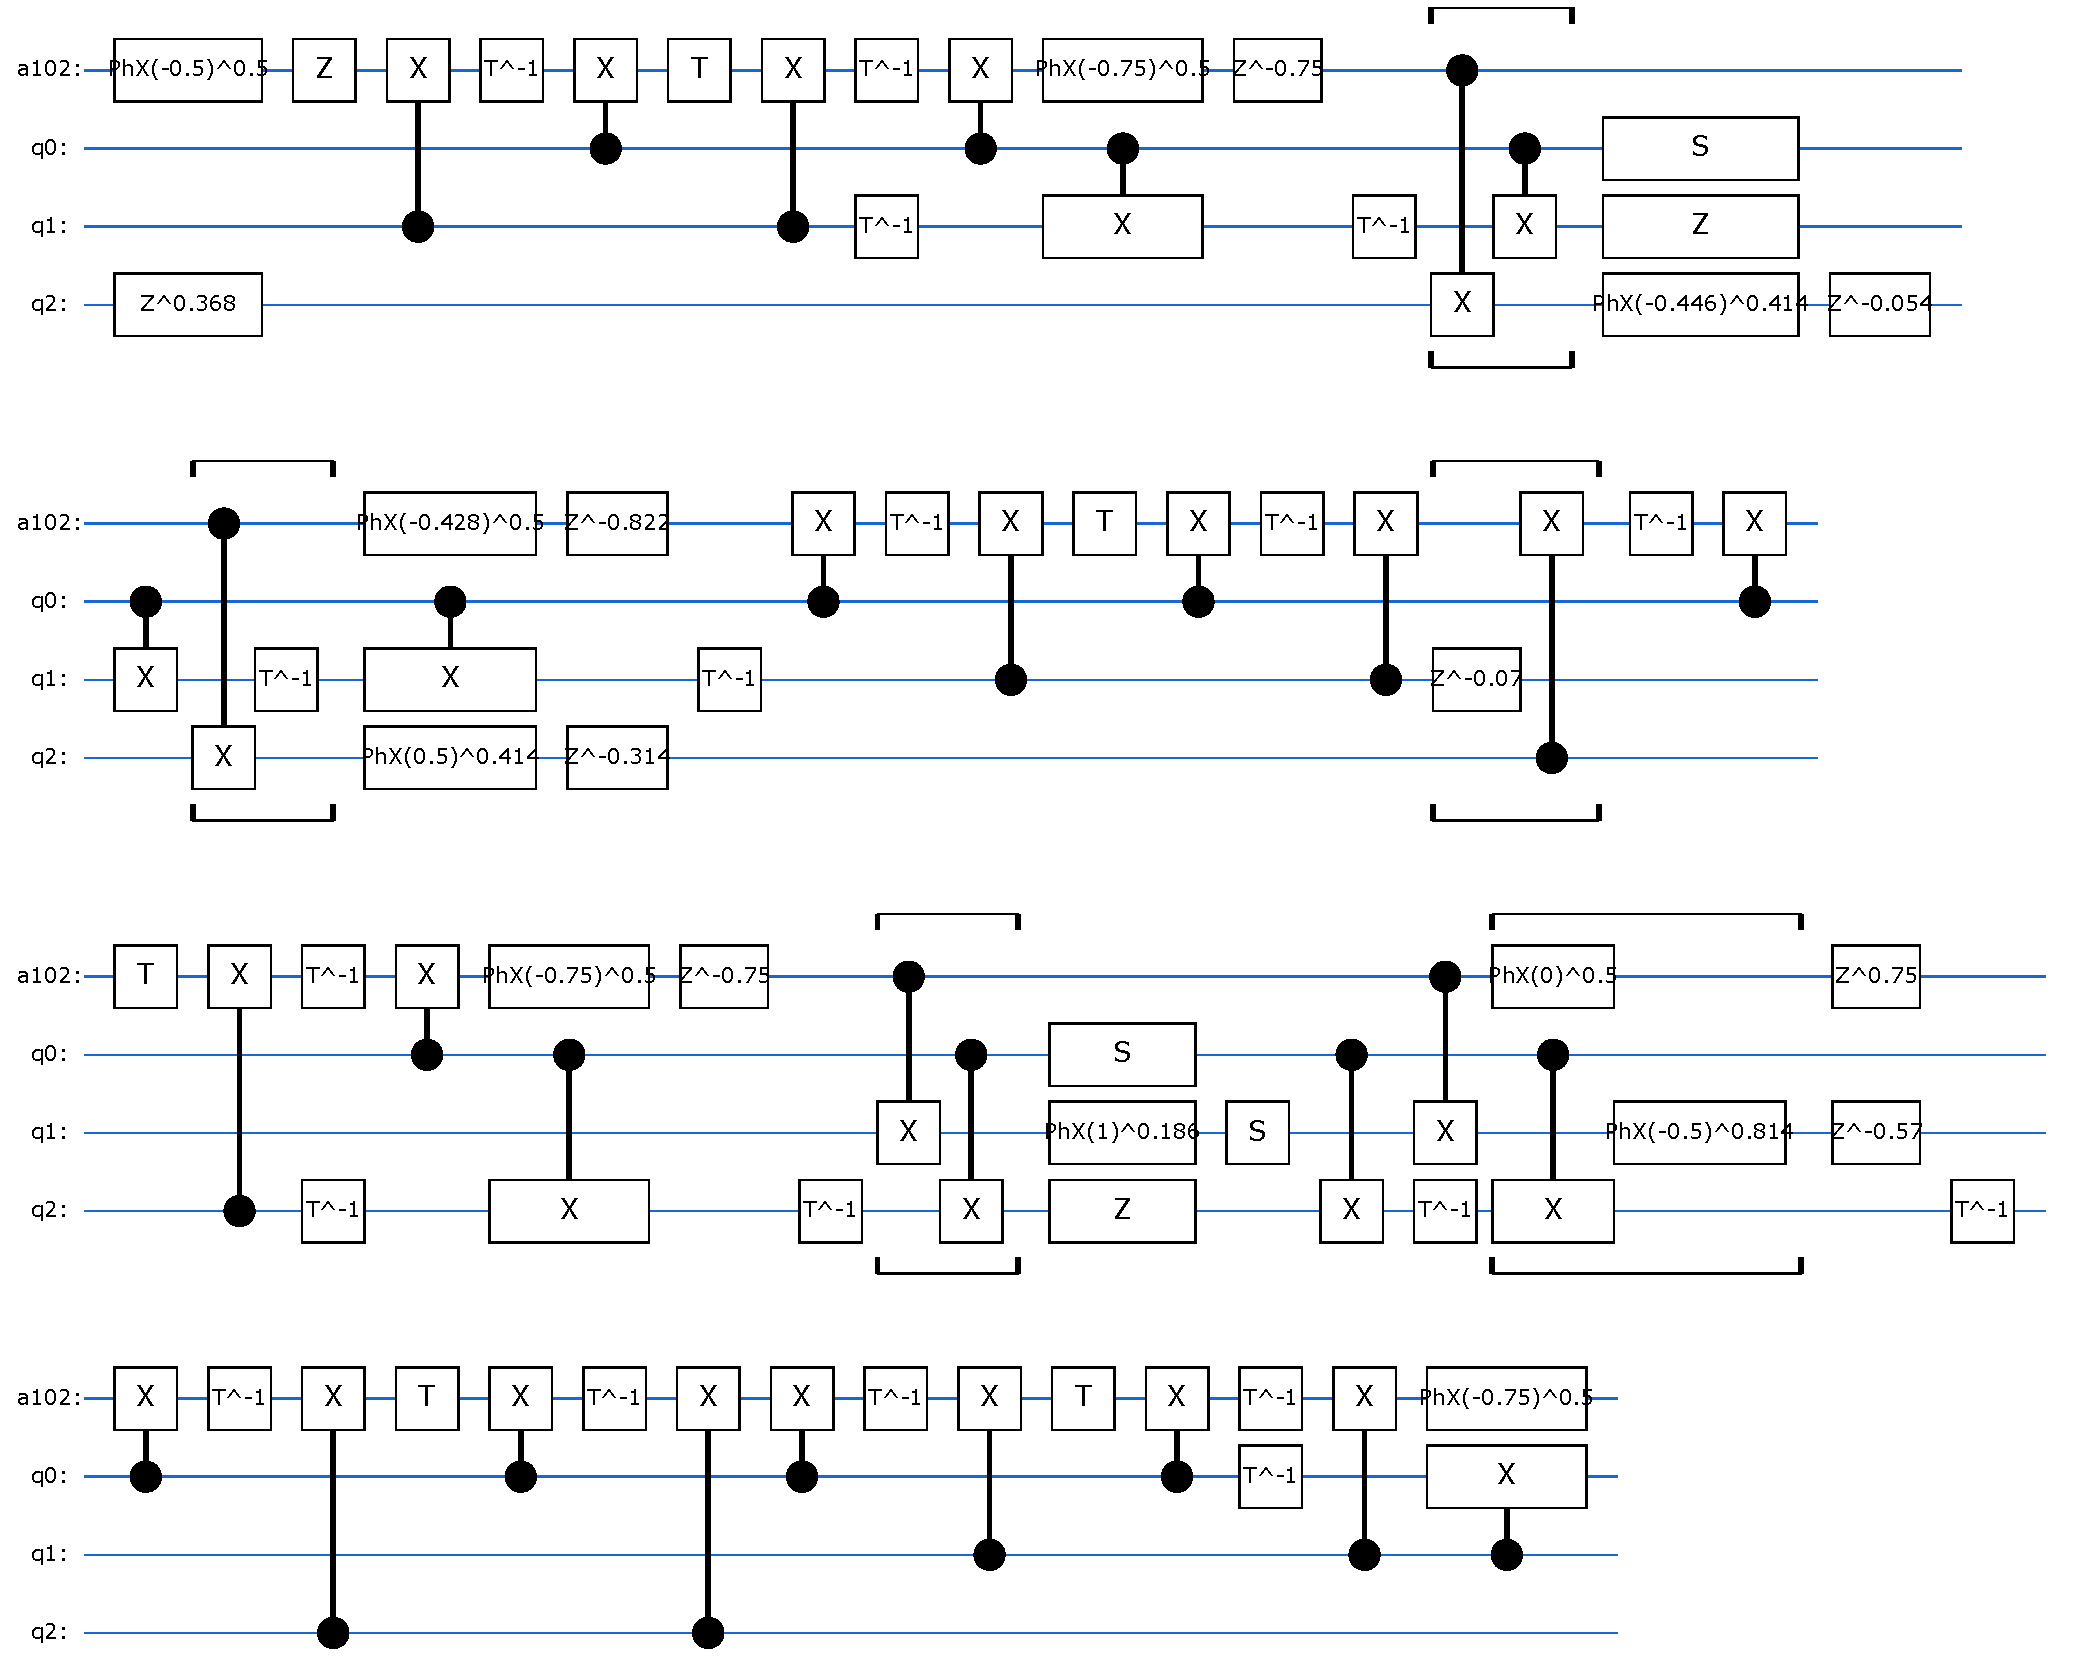
\includegraphics[width=\textwidth]{cirq-circuit.pdf}
                            \caption{Circuit diagram (partial) in Cirq\texttrademark.}
                            \label{fig:cirq-circuit}
                        \end{subfigure}
                        \caption{Quantum evolution compiled once and quantum circuit rendered multiple times.}
                        \label{fig:circuit-example}
                    \end{figure}

                \end{block}
            \end{column}

            % Column 3
            \begin{column}{0.33\textwidth}
                \begin{block}{Results}

                    For illustration, we created an evolution operator from a randomly generating a $8 \times 8$ unitary matrix
                    \begin{equation}
                        \label{eq:random-mat}
                        U =
                        \begin{bmatrix}
                            0.2246+0.3674j & 0.0756+0.3213j & \dots & -0.0534-0.1667j & -0.3321-0.1199j \\
                            -0.2123-0.0162j & 0.115+0.4483j & \dots & -0.1772-0.1398j & -0.1267+0.3692j \\
                            \vdots & \vdots & \ddots & \vdots & \vdots \\
                            0.1554+0.0272j & -0.4272+0.5894j & \dots & 0.1361+0.1934j & 0.3972+0.3205j \\
                            -0.3795+0.3577j & -0.0237-0.1054j & \dots & 0.0838-0.4389j & 0.1242-0.0068j
                        \end{bmatrix}.
                    \end{equation}


                    We choose \texttt{PRINCIPAL} as the compilation granularity.
                    The evolution operator is compiled and stored the compiled QIL in a \texttt{.qco} file.
                    Figure~\ref{fig:circuit-example} displays the circuit diagrams in Qiskit and Cirq, both
                    are rendered from the same QIL\@.
                    We also transpiled the compiled code from QIL to OpenQASM~\cite{openqasm2,openqasm3}
                    The generated \texttt{QASM} code is similar to Listing~\ref{lst:qasm} which we will not repeat.


                    % Top horizontal line
                    \noindent\rule{\linewidth}{0.5pt}
                    \vspace{0.5em}
                    \begin{minipage}{0.48\linewidth}
                        \inputminted[
                            linenos,
                            xleftmargin=2em,
                            firstline=1,
                            lastline=12,
                        ]{asm}{code.qasm}
                        \label{lst:qasm}
                    \end{minipage}\hfill
                    \begin{minipage}{0.48\linewidth}
                        \inputminted[
                            linenos,
                            xleftmargin=2em,
                            firstline=13,
                        ]{asm}{code.qasm}
                    \end{minipage}
                    \noindent\rule{\linewidth}{0.5pt}
                \end{block}

                \begin{block}{Conclusion}
                    We have presented \texttt{Qompiler}, a traceable and verifiable quantum circuit synthesizer that bridges the gap between physics-based Hamiltonian modeling
                    and cross-platform quantum software development.
                    By leveraging a configurable, multi-stage decomposition framework and a B-Tree intermediate representation,
                    \texttt{Qompiler} enables gate-level lineage tracking and hardware-aware circuit synthesis.
                    The platform-agnostic design allows seamless rendering of circuits into backends such as Qiskit, Cirq,
                    and OpenQASM, promoting broad compatibility and flexible deployment.
                    Importantly, the compiler’s fine-grained control over gate type selection empowers users to optimize circuits for the unique characteristics of
                    various quantum hardware platforms. \texttt{Qompiler} provides a scalable, transparent,
                    and adaptable solution that supports efficient quantum algorithm development across the heterogeneous quantum computing landscape.


                    \vspace{1em}
                    \qrcode{https://github.com/wanshoupu/quantum-simulations}

                    \vspace{1em}
                    \texttt{github.com/wanshoupu/quantum-simulations}

                    \textbf{Feedback and collaboration welcome!}
                \end{block}

                \begin{block}{References}
                    \begin{thebibliography}{99}
                        \bibitem{tket} S. Sivarajah \textit{et al.}, ``t|ket⟩: A Retargetable Compiler for NISQ Devices,'' arXiv preprint arXiv.2003.10611, 2020.

                        \bibitem{quilc} Rigetti Computing, ``An Open-Source, Industrial-Strength Optimizing Compiler for Quantum Programs,'' arXiv preprint arXiv:2003.13961, 2020.
                        Available: https://github.com/rigetti/quilc.

                        \bibitem{qfast} E. Younis \textit{et al.}, ``QFAST: Quantum Synthesis Using a Hierarchical Continuous Circuit Space,'' arXiv preprint arXiv.2003.04462, 2020.

                        \bibitem{staq} M. Amy \textit{et al.}, ``Staq: A Full-Stack Quantum Processing Toolkit,'' in Quantum Science and Technology, Focus on Quantum Software, 5, 034016 (2020).
                        arXiv preprint arXiv.1912.06070, 2020.

                        \bibitem{nielsen2010quantum}
                        M. A. Nielsen and I. L. Chuang, \textit{Quantum Computation and Quantum Information}, Cambridge Univ. Press, 2010.

                        \bibitem{openqasm2} A. W. Cross \textit{et al.}, ``Open Quantum Assembly Language,'' arXiv preprint arXiv:1707.03429, 2017.

                        \bibitem{openqasm3} A. W. Cross \textit{et al.}, ``OpenQASM 3: A broader and deeper quantum assembly language,'' arXiv preprint arXiv:2104.14722, 2021.
                    \end{thebibliography}
                \end{block}
            \end{column}

        \end{columns}

    \end{frame}

\end{document}
